\documentclass{ximera}

 

\usepackage{epsfig}

\graphicspath{
  {./}
  {figures/}
}

\usepackage{morewrites}
\makeatletter
\newcommand\subfile[1]{%
\renewcommand{\input}[1]{}%
\begingroup\skip@preamble\otherinput{#1}\endgroup\par\vspace{\topsep}
\let\input\otherinput}
\makeatother

\newcommand{\includeexercises}{\directlua{dofile("/home/jim/linearAlgebra/laode/exercises.lua")}}

%\newcounter{ccounter}
%\setcounter{ccounter}{1}
%\newcommand{\Chapter}[1]{\setcounter{chapter}{\arabic{ccounter}}\chapter{#1}\addtocounter{ccounter}{1}}

%\newcommand{\section}[1]{\section{#1}\setcounter{thm}{0}\setcounter{equation}{0}}

%\renewcommand{\theequation}{\arabic{chapter}.\arabic{section}.\arabic{equation}}
%\renewcommand{\thefigure}{\arabic{chapter}.\arabic{figure}}
%\renewcommand{\thetable}{\arabic{chapter}.\arabic{table}}

%\newcommand{\Sec}[2]{\section{#1}\markright{\arabic{ccounter}.\arabic{section}.#2}\setcounter{equation}{0}\setcounter{thm}{0}\setcounter{figure}{0}}

\newcommand{\Sec}[2]{\section{#1}}

\setcounter{secnumdepth}{2}
%\setcounter{secnumdepth}{1} 

%\newcounter{THM}
%\renewcommand{\theTHM}{\arabic{chapter}.\arabic{section}}

\newcommand{\trademark}{{R\!\!\!\!\!\bigcirc}}
%\newtheorem{exercise}{}

\newcommand{\dfield}{{\sf dfield9}}
\newcommand{\pplane}{{\sf pplane9}}

\newcommand{\EXER}{\section*{Exercises}}%\vspace*{0.2in}\hrule\small\setcounter{exercise}{0}}
\newcommand{\CEXER}{}%\vspace{0.08in}\begin{center}Computer Exercises\end{center}}
\newcommand{\TEXER}{} %\vspace{0.08in}\begin{center}Hand Exercises\end{center}}
\newcommand{\AEXER}{} %\vspace{0.08in}\begin{center}Hand Exercises\end{center}}

% BADBAD: \newcommand{\Bbb}{\bf}

\newcommand{\R}{\mbox{$\Bbb{R}$}}
\newcommand{\C}{\mbox{$\Bbb{C}$}}
\newcommand{\Z}{\mbox{$\Bbb{Z}$}}
\newcommand{\N}{\mbox{$\Bbb{N}$}}
\newcommand{\D}{\mbox{{\bf D}}}
\usepackage{amssymb}
%\newcommand{\qed}{\hfill\mbox{\raggedright$\square$} \vspace{1ex}}
%\newcommand{\proof}{\noindent {\bf Proof:} \hspace{0.1in}}

\newcommand{\setmin}{\;\mbox{--}\;}
\newcommand{\Matlab}{{M\small{AT\-LAB}} }
\newcommand{\Matlabp}{{M\small{AT\-LAB}}}
\newcommand{\computer}{\Matlab Instructions}
\newcommand{\half}{\mbox{$\frac{1}{2}$}}
\newcommand{\compose}{\raisebox{.15ex}{\mbox{{\scriptsize$\circ$}}}}
\newcommand{\AND}{\quad\mbox{and}\quad}
\newcommand{\vect}[2]{\left(\begin{array}{c} #1_1 \\ \vdots \\
 #1_{#2}\end{array}\right)}
\newcommand{\mattwo}[4]{\left(\begin{array}{rr} #1 & #2\\ #3
&#4\end{array}\right)}
\newcommand{\mattwoc}[4]{\left(\begin{array}{cc} #1 & #2\\ #3
&#4\end{array}\right)}
\newcommand{\vectwo}[2]{\left(\begin{array}{r} #1 \\ #2\end{array}\right)}
\newcommand{\vectwoc}[2]{\left(\begin{array}{c} #1 \\ #2\end{array}\right)}

\newcommand{\ignore}[1]{}


\newcommand{\inv}{^{-1}}
\newcommand{\CC}{{\cal C}}
\newcommand{\CCone}{\CC^1}
\newcommand{\Span}{{\rm span}}
\newcommand{\rank}{{\rm rank}}
\newcommand{\trace}{{\rm tr}}
\newcommand{\RE}{{\rm Re}}
\newcommand{\IM}{{\rm Im}}
\newcommand{\nulls}{{\rm null\;space}}

\newcommand{\dps}{\displaystyle}
\newcommand{\arraystart}{\renewcommand{\arraystretch}{1.8}}
\newcommand{\arrayfinish}{\renewcommand{\arraystretch}{1.2}}
\newcommand{\Start}[1]{\vspace{0.08in}\noindent {\bf Section~\ref{#1}}}
\newcommand{\exer}[1]{\noindent {\bf \ref{#1}}}
\newcommand{\ans}{}
\newcommand{\matthree}[9]{\left(\begin{array}{rrr} #1 & #2 & #3 \\ #4 & #5 & #6
\\ #7 & #8 & #9\end{array}\right)}
\newcommand{\cvectwo}[2]{\left(\begin{array}{c} #1 \\ #2\end{array}\right)}
\newcommand{\cmatthree}[9]{\left(\begin{array}{ccc} #1 & #2 & #3 \\ #4 & #5 &
#6 \\ #7 & #8 & #9\end{array}\right)}
\newcommand{\vecthree}[3]{\left(\begin{array}{r} #1 \\ #2 \\
#3\end{array}\right)}
\newcommand{\cvecthree}[3]{\left(\begin{array}{c} #1 \\ #2 \\
#3\end{array}\right)}
\newcommand{\cmattwo}[4]{\left(\begin{array}{cc} #1 & #2\\ #3
&#4\end{array}\right)}

\newcommand{\Matrix}[1]{\ensuremath{\left(\begin{array}{rrrrrrrrrrrrrrrrrr} #1 \end{array}\right)}}

\newcommand{\Matrixc}[1]{\ensuremath{\left(\begin{array}{cccccccccccc} #1 \end{array}\right)}}



\renewcommand{\labelenumi}{\theenumi)}
\newenvironment{enumeratea}%
{\begingroup
 \renewcommand{\theenumi}{\alph{enumi}}
 \renewcommand{\labelenumi}{(\theenumi)}
 \begin{enumerate}}
 {\end{enumerate}\endgroup}



\newcounter{help}
\renewcommand{\thehelp}{\thesection.\arabic{equation}}

%\newenvironment{equation*}%
%{\renewcommand\endequation{\eqno (\theequation)* $$}%
%   \begin{equation}}%
%   {\end{equation}\renewcommand\endequation{\eqno \@eqnnum
%$$\global\@ignoretrue}}

%\input{psfig.tex}

\author{Martin Golubitsky and Michael Dellnitz}

%\newenvironment{matlabEquation}%
%{\renewcommand\endequation{\eqno (\theequation*) $$}%
%   \begin{equation}}%
%   {\end{equation}\renewcommand\endequation{\eqno \@eqnnum
% $$\global\@ignoretrue}}

\newcommand{\soln}{\textbf{Solution:} }
\newcommand{\exercap}[1]{\centerline{Figure~\ref{#1}}}
\newcommand{\exercaptwo}[1]{\centerline{Figure~\ref{#1}a\hspace{2.1in}
Figure~\ref{#1}b}}
\newcommand{\exercapthree}[1]{\centerline{Figure~\ref{#1}a\hspace{1.2in}
Figure~\ref{#1}b\hspace{1.2in}Figure~\ref{#1}c}}
\newcommand{\para}{\hspace{0.4in}}

\renewenvironment{solution}{\suppress}{\endsuppress}

\ifxake
\newenvironment{matlabEquation}{\begin{equation}}{\end{equation}}
\else
\newenvironment{matlabEquation}%
{\let\oldtheequation\theequation\renewcommand{\theequation}{\oldtheequation*}\begin{equation}}%
  {\end{equation}\let\theequation\oldtheequation}
\fi

\makeatother


\title{The Geometry of Low-Dimensional Solutions}

\begin{document}
\begin{abstract}
\end{abstract}
\maketitle


\label{S:2.2}

In this section we discuss how to use \Matlab graphics to solve
systems of linear equations in two and three unknowns.  We begin
with two dimensions.

\subsection*{Linear Equations in Two Dimensions}

The set of all solutions to the equation
\begin{equation} \label{2x-y=6}
2x - y = 6
\end{equation}
is a straight line in the $xy$ plane; this line
has slope $2$ and $y$-intercept equal to $-6$.  We can use
\Matlab to plot the solutions to this equation --- though some
understanding of the way \Matlab works is needed.

The {\tt plot} command in \Matlab plots a sequence of points in
the plane, as follows.  Let $X$ and $Y$ be $n$ vectors. Then
\begin{verbatim}
plot(X,Y)
\end{verbatim} \index{\computer!plot}
will plot the points $(X(1),Y(1))$, $(X(2),Y(2))$, \ldots,
$(X(n),Y(n))$ in the $xy$-plane.  

To plot points on the line
\eqref{2x-y=6} we need to enter the $x$-coordinates of the points
we wish to plot.  If we want to plot a hundred points, we would
be facing a tedious task.  \Matlab has a command to simplify
this task. Typing
\begin{verbatim}
x = linspace(-5,5,100);
\end{verbatim} \index{\computer!linspace}
produces a vector $x$ with $100$ entries with the $1^{st}$ entry
equal to $-5$, the last entry equal to $5$, and the remaining $98$ 
entries equally spaced between $-5$ and $5$.  \Matlab has another command 
that allows us to create a vector of points {\tt x}.  In this command
we specify the distance between points rather than the number of 
points.  That command is:
\begin{verbatim}
x = -5:0.1:5;
\end{verbatim}
Producing {\tt x} by either command is acceptable.

Typing
\begin{verbatim}
y = 2*x - 6;
\end{verbatim}
produces a vector whose entries correspond to the
$y$-coordinates of points on the line \eqref{2x-y=6}.  Then typing
\begin{verbatim}
plot(x,y)
\end{verbatim}
produces the desired plot.  It is useful to label the axes on
this figure, which is accomplished by typing
\begin{verbatim}
xlabel('x')
ylabel('y')
\end{verbatim} \index{\computer!xlabel}\index{\computer!ylabel}

We can now use \Matlab to solve the equation \eqref{small}
graphically.  Recall that \eqref{small} is:
\[
\arraycolsep 2pt
\begin{array}{rcrcr}
 x & + &  y & = & 7 \\
-x & + & 3y & = & 1
\end{array}
\]
A solution to this system of equations is a point that lies on
both lines in the system.  Suppose that we search for a solution
to this system that has an $x$-coordinate between $-3$ and $7$.
Then type the commands
\begin{verbatim}
x = linspace(-3,7,100);
y = 7 - x;
plot(x,y)
xlabel('x')
ylabel('y')
hold on
y = (1 + x)/3;
plot(x,y)
axis('equal')
grid
\end{verbatim} \index{\computer!hold} \index{\computer!axis('equal')}
\index{\computer!grid}
The \Matlab command {\tt hold on} tells \Matlab to keep the
present figure and to add the information that follows to that figure.
The command {\tt axis('equal')} instructs \Matlab to make unit distances
on the $x$ and $y$ axes equal.  The last \Matlab command superimposes
grid lines. See Figure~\ref{lineint}.  From this figure
you can see that the solution to this system is $(x,y)=(5,2)$, which
we already knew.

\begin{figure}[htb]
                       \centerline{%
                       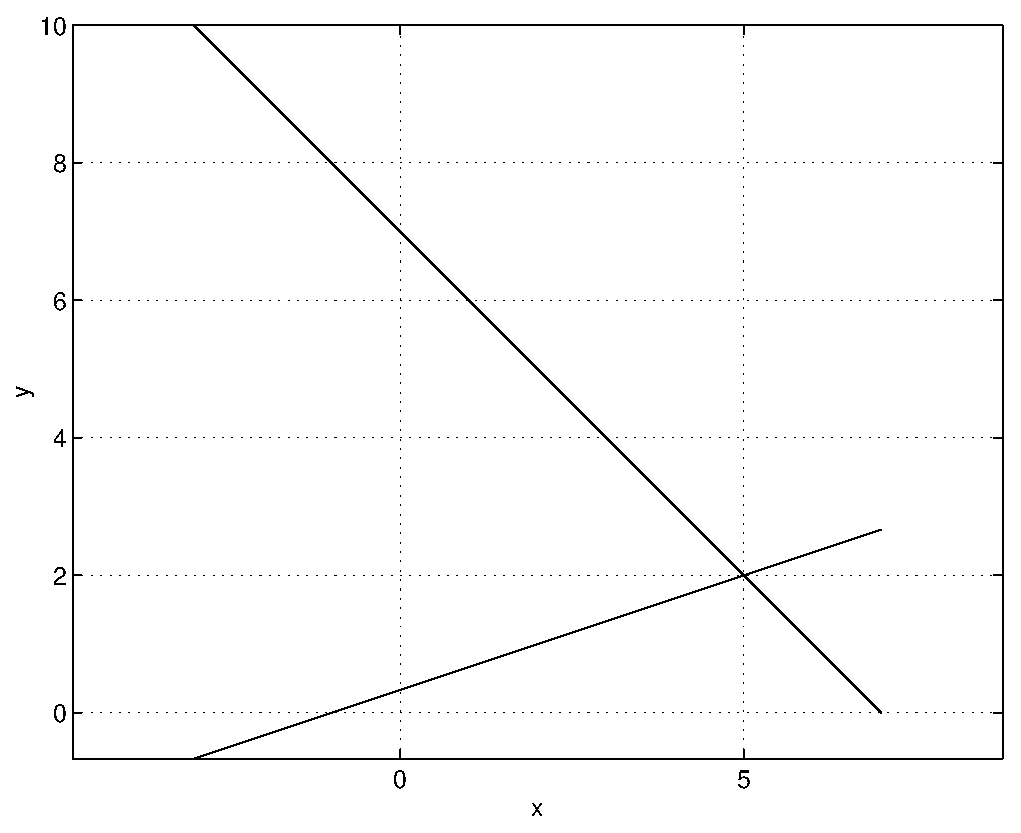
\psfig{file=../figures/lineint.eps,width=3.5in}}
                       \caption{Graph of equations in \protect\eqref{small}}
                       \label{lineint}
\end{figure}


There are several principles that follow from this exercise.
\begin{itemize}
\item   Solutions to a single linear equation in two variables
form a straight line.
\item Solutions to two linear equations in two unknowns lie at
the intersection of two straight lines in the plane.
\end{itemize}
It follows that the solution to two linear equations in two
variables is a single point if the lines are not parallel.  If
these lines are parallel and unequal, then there are no
solutions, as there are no points of intersection.

\subsection*{Linear Equations in Three Dimensions}

We begin by observing that the set of all solutions to a linear
equation in three variables forms a plane\index{plane}.  More
precisely, the solutions to the equation
\begin{equation} \label{abcd}
ax+by+cz=d
\end{equation}
form a plane that is perpendicular to the vector $(a,b,c)$ ---
assuming of course that the vector $(a,b,c)$ is nonzero.

This fact is most easily proved using the {\em dot product\/}.
Recall from Chapter~\ref{chap:prelim} \eqref{e:dotproduct} that
the dot product\index{dot product} is defined by
\[
X\cdot Y = x_1y_1+x_2y_2+x_3y_3,
\]
where $X=(x_1,x_2,x_3)$ and $Y=(y_1,y_2,y_3)$.  We recall from
Chapter~\ref{chap:prelim} \eqref{dotprod=0} the following important
fact concerning dot products:
\[
X\cdot Y = 0
\]
if and only if the vectors $X$ and $Y$ are perpendicular.

Suppose that $N=(a,b,c)\neq 0$.  Consider the plane that is perpendicular
to the {\em normal vector\/}\index{normal vector} $N$ and that contains the
point $X_0$.  If the point $X$ lies in that plane, then $X-X_0$ is
perpendicular to $N$; that is,
\begin{equation} \label{XX_0}
(X-X_0)\cdot N = 0.
\end{equation}
If we use the notation
\[
X=(x,y,z) \quad \mbox{ and } \quad X_0=(x_0,y_0,z_0),
\]
then \eqref{XX_0} becomes
\[
a(x-x_0)+b(y-y_0)+c(z-z_0)=0.
\]
Setting
\[
d=ax_0 + by_0 + cz_0
\]
puts equation \eqref{XX_0} into the form \eqref{abcd}.  In this way
we see that the set of solutions to a single linear equation in
three variables forms a plane.  See Figure~\ref{F:plane}.

\begin{figure}[htb]
              \centerline{%
              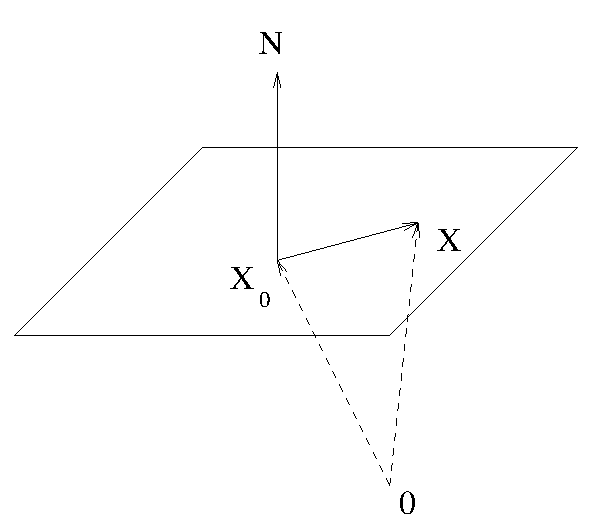
\psfig{file=../figures/plane.eps,width=2.5in}}
              \caption{The plane containing $X_0$ and perpendicular to $N$.}
              \label{F:plane}
\end{figure}


We now use \Matlab to visualize the planes that are solutions to
linear equations.  Plotting an equation in three dimensions in
\Matlab follows a structure similar to the planar plots.
Suppose that we wish to plot the solutions to the equation
\begin{equation} \label{-2x+3y+z=2}
-2x+3y+z=2.
\end{equation}
We can rewrite \eqref{-2x+3y+z=2} as
\[
z=2x-3y+2.
\]
It is this function that we actually graph by typing the
commands
\begin{verbatim}
[x,y] = meshgrid(-5:0.5:5);
z = 2*x - 3*y + 2;
surf(x,y,z)
\end{verbatim} \index{\computer!meshgrid}  \index{\computer!surf}
The first command tells \Matlab to create a square grid in the
$xy$-plane.  Grid points are
equally spaced between $-5$ and $5$ at intervals of $0.5$ on
both the $x$ and $y$ axes. The second command tells \Matlab to
compute the $z$ value of the solution to \eqref{-2x+3y+z=2} at
each grid point.  The third command tells \Matlab to graph the
surface containing the points $(x,y,z)$.  See
Figure~\ref{F:p1int}.

\begin{figure}[htb]
              \centerline{%
              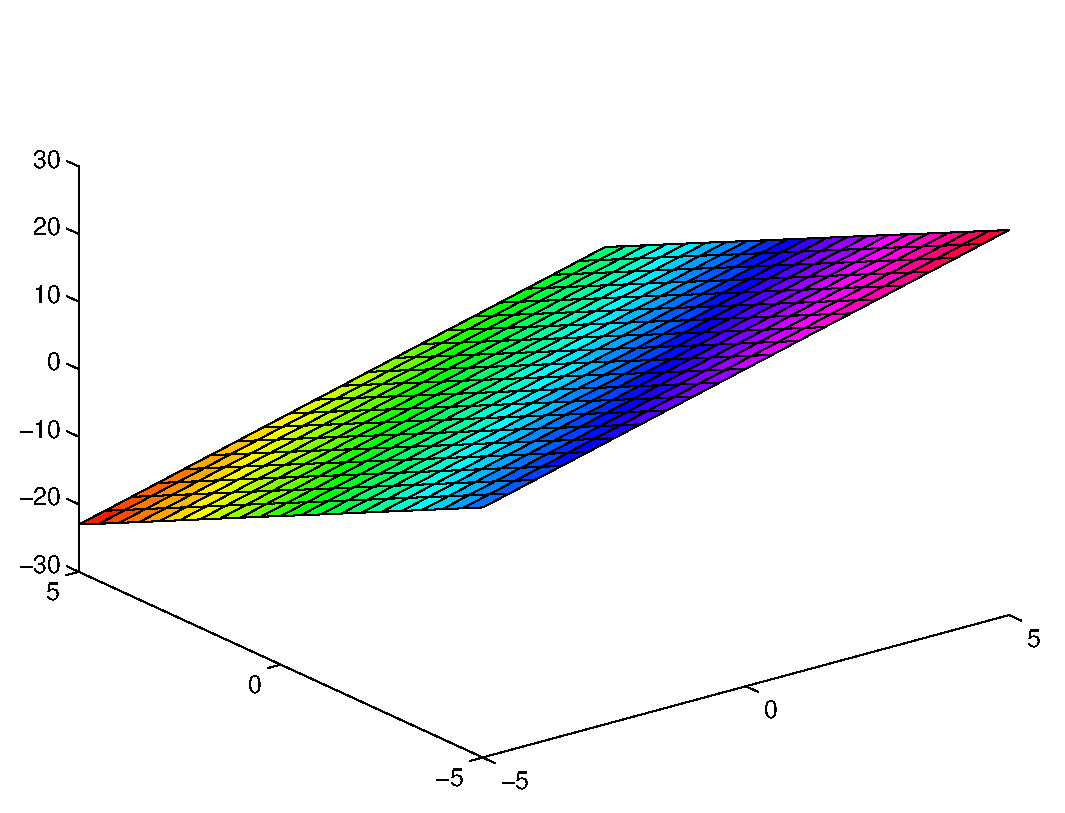
\psfig{file=../figures/p1int.eps,width=3.0in}}
              \caption{Graph of \protect\eqref{-2x+3y+z=2}.}
              \label{F:p1int}
\end{figure}


We can now see that solutions to a system of two linear
equations in three unknowns consists of points that lie
simultaneously on two planes.  As long as the normal vectors to
these planes are not parallel, the intersection of the two
planes will be a line in three dimensions.  Indeed, consider the
equations
\begin{eqnarray*}
-2x + 3y + z & = & 2 \\
 2x - 3y + z & = & 0.
\end{eqnarray*}
We can graph the solution using \Matlab, as follows. We continue
from the previous graph by typing
\begin{verbatim}
hold on
z = -2*x + 3*y;
surf(x,y,z)
\end{verbatim}
The result, which illustrates that the intersection of two planes
in $\R^3$ is generally a line, is shown in Figure~\ref{F:p2int}.

\begin{figure}[htb]
              \centerline{%
              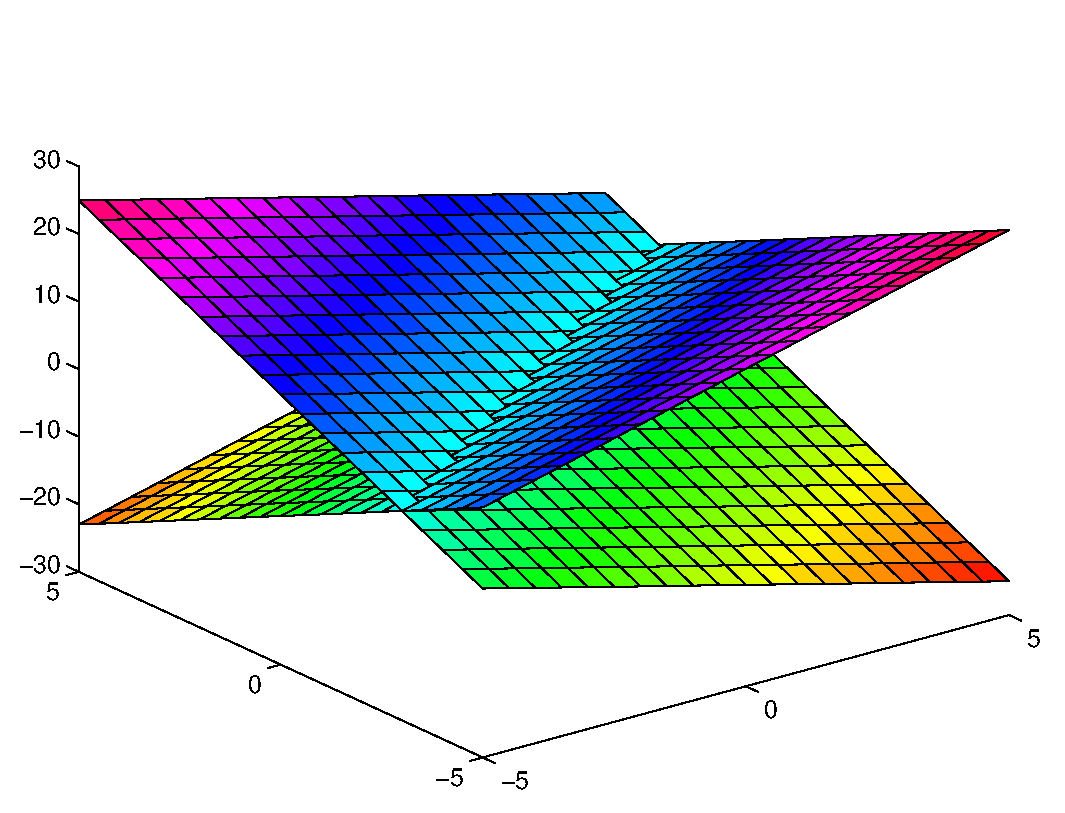
\psfig{file=../figures/p2int.eps,width=3.0in}}
              \caption{Line of intersection of two planes.}
              \label{F:p2int}
\end{figure}

We can now see geometrically that the solution to three
simultaneous linear equations in three unknowns will generally
be a point --- since generally three planes in three space
intersect in a point.  To visualize this intersection, as shown in
Figure~\ref{F:p3int}, we extend the previous system of equations to
\begin{eqnarray*}
-2x +   3y + z & = & 2 \\
 2x -   3y + z & = & 0\\
-3x + 0.2y + z & = & 1.
\end{eqnarray*}
Continuing in \Matlab type
\begin{verbatim}
z = 3*x - 0.2*y + 1;
surf(x,y,z)
\end{verbatim}

\begin{figure}[htb]
              \centerline{%
              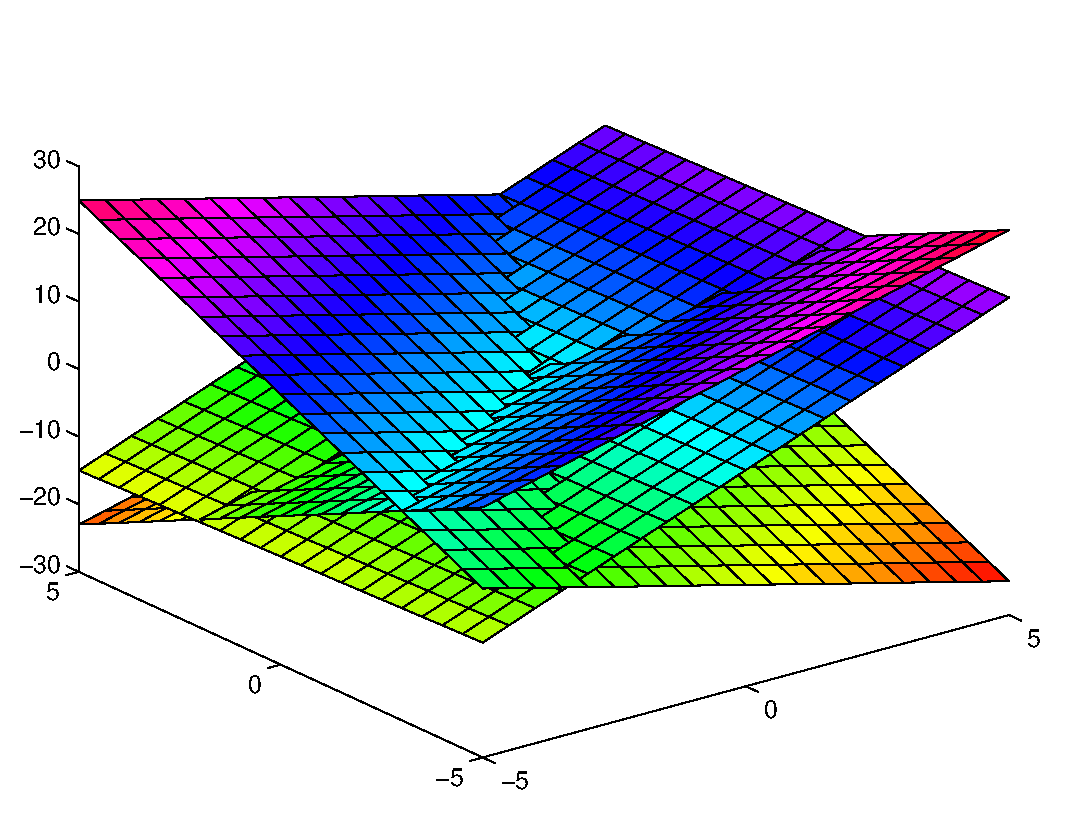
\psfig{file=../figures/p3int.eps,width=3.0in}}
              \caption{Point of intersection of three planes.}
              \label{F:p3int}
\end{figure}

Unfortunately, visualizing the point of intersection of these
planes geometrically does not really help to get an accurate
numerical value of the coordinates of this intersection point.  
However, we can use \Matlab to solve this system accurately.
Denote the $3\times 3$ matrix of coefficients by {\tt A}, the 
vector of coefficients on the right hand side by {\tt b}, and 
the solution by {\tt x}.  Solve the system in \Matlab by typing
\begin{verbatim}
A = [ -2 3 1; 2 -3 1; -3 0.2 1];
b = [2; 0; 1];
x = A\b
\end{verbatim}
The point of intersection of the three planes is at
\begin{verbatim}
x =
    0.0233
    0.3488
    1.0000
\end{verbatim}

Three planes in three dimensional space need not intersect in a
single point.  For example, if two of the planes are parallel
they need not intersect at all.  The normal vectors must point
in {\em independent\/} directions to
guarantee that the intersection is a point.  Understanding the
notion of independence (it is more complicated than just not
being parallel) is part of the subject of linear algebra.
\Matlab returns ``{\tt Inf}'', which we have seen previously,
when these normal vectors are (approximately) dependent. For
example, consider Exercise~\ref{c2.2.10}.

\subsection*{Plotting Nonlinear Functions in \Matlab}

Suppose that we want to plot the graph of a nonlinear function of
a single variable, such as
\begin{equation}  \label{E:quadex}
y = x^2 - 2x + 3
\end{equation}
on the interval $[-2,5]$ using \Matlabp.  There is a difficulty:  How
do we enter the term $x^2$?  For example, suppose that we type
\begin{verbatim}
x = linspace(-2,5);
y = x*x - 2*x + 3;
\end{verbatim}
Then \Matlab responds with
\begin{verbatim}
??? Error using ==> *
Inner matrix dimensions must agree.
\end{verbatim}
The problem is that in \Matlab the variable {\tt x} is a vector of
100 equally spaced points {\tt x(1), x(2), \ldots, x(100)}.  What we
really need is a vector consisting of entries {\tt x(1)*x(1), x(2)*x(2),
\ldots, x(100)*x(100)}.  \Matlab has the facility to perform this
operation automatically and the syntax for the operation is {\tt .*}
rather than {\tt *}.  So typing
\begin{verbatim}
x = linspace(-2,5);
y = x.*x - 2*x + 3;
plot(x,y)
\end{verbatim}\index{\computer!{\tt .*}}
produces the graph of \eqref{E:quadex} in Figure~\ref{F:quadex}.
\begin{figure}[htb]
              \centerline{%
              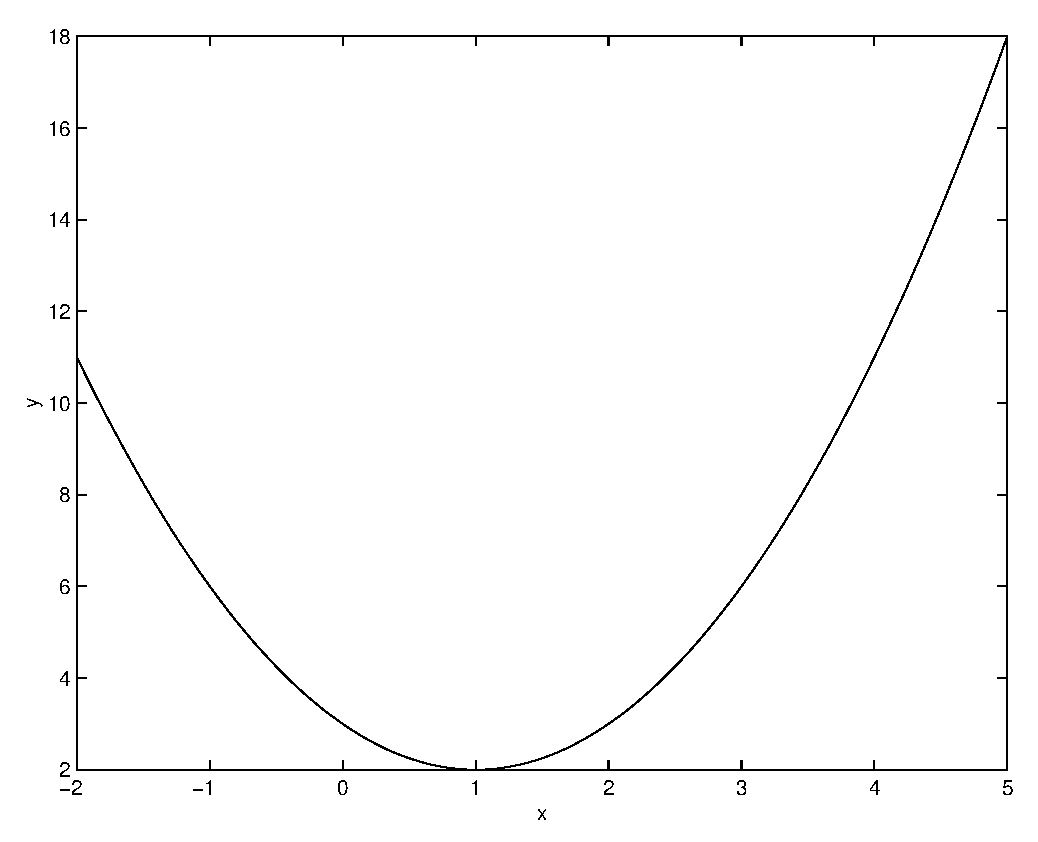
\psfig{file=../figures/quadex.eps,width=3.0in}}
              \caption{Graph of $y = x^2 - 2x + 3$.}
              \label{F:quadex}
\end{figure}
In a similar fashion, \Matlab has the `dot' operations of
{\tt ./}\index{\computer!{\tt ./}},
{\tt .$\backslash$}, and  .\^{}\index{\computer!.\^{}}, as well
as {\tt .*}.



\includeexercises


\end{document}
